% Options for packages loaded elsewhere
\PassOptionsToPackage{unicode}{hyperref}
\PassOptionsToPackage{hyphens}{url}
\PassOptionsToPackage{dvipsnames,svgnames*,x11names*}{xcolor}
%
\documentclass[
]{article}
\usepackage{lmodern}
\usepackage{amssymb,amsmath}
\usepackage{ifxetex,ifluatex}
\ifnum 0\ifxetex 1\fi\ifluatex 1\fi=0 % if pdftex
  \usepackage[T1]{fontenc}
  \usepackage[utf8]{inputenc}
  \usepackage{textcomp} % provide euro and other symbols
\else % if luatex or xetex
  \usepackage{unicode-math}
  \defaultfontfeatures{Scale=MatchLowercase}
  \defaultfontfeatures[\rmfamily]{Ligatures=TeX,Scale=1}
\fi
% Use upquote if available, for straight quotes in verbatim environments
\IfFileExists{upquote.sty}{\usepackage{upquote}}{}
\IfFileExists{microtype.sty}{% use microtype if available
  \usepackage[]{microtype}
  \UseMicrotypeSet[protrusion]{basicmath} % disable protrusion for tt fonts
}{}
\makeatletter
\@ifundefined{KOMAClassName}{% if non-KOMA class
  \IfFileExists{parskip.sty}{%
    \usepackage{parskip}
  }{% else
    \setlength{\parindent}{0pt}
    \setlength{\parskip}{6pt plus 2pt minus 1pt}}
}{% if KOMA class
  \KOMAoptions{parskip=half}}
\makeatother
\usepackage{xcolor}
\IfFileExists{xurl.sty}{\usepackage{xurl}}{} % add URL line breaks if available
\IfFileExists{bookmark.sty}{\usepackage{bookmark}}{\usepackage{hyperref}}
\hypersetup{
  pdftitle={Modern Data Mining, HW 1},
  pdfauthor={Sarah Hayward; Annie Vo; Jessica Brown},
  colorlinks=true,
  linkcolor=Maroon,
  filecolor=Maroon,
  citecolor=Blue,
  urlcolor=blue,
  pdfcreator={LaTeX via pandoc}}
\urlstyle{same} % disable monospaced font for URLs
\usepackage[margin=1in]{geometry}
\usepackage{graphicx,grffile}
\makeatletter
\def\maxwidth{\ifdim\Gin@nat@width>\linewidth\linewidth\else\Gin@nat@width\fi}
\def\maxheight{\ifdim\Gin@nat@height>\textheight\textheight\else\Gin@nat@height\fi}
\makeatother
% Scale images if necessary, so that they will not overflow the page
% margins by default, and it is still possible to overwrite the defaults
% using explicit options in \includegraphics[width, height, ...]{}
\setkeys{Gin}{width=\maxwidth,height=\maxheight,keepaspectratio}
% Set default figure placement to htbp
\makeatletter
\def\fps@figure{htbp}
\makeatother
\setlength{\emergencystretch}{3em} % prevent overfull lines
\providecommand{\tightlist}{%
  \setlength{\itemsep}{0pt}\setlength{\parskip}{0pt}}
\setcounter{secnumdepth}{5}

\title{Modern Data Mining, HW 1}
\author{Sarah Hayward \and Annie Vo \and Jessica Brown}
\date{Due: 11:59PM, Jan.~30th, 2021}

\begin{document}
\maketitle

{
\hypersetup{linkcolor=}
\setcounter{tocdepth}{4}
\tableofcontents
}
\pagebreak

\hypertarget{overview}{%
\section{Overview}\label{overview}}

This is a fast-paced course that covers a lot of material. There will be
a large amount of references. You may need to do your own research to
fill in the gaps in between lectures and homework/projects. It is
impossible to learn data science without getting your hands dirty.
Please budget your time evenly. Last-minute work ethic will not work for
this course.

Homework in this course is different from your usual homework assignment
as a typical student. Most of the time, they are built over real case
studies. While you will be applying methods covered in lectures, you
will also find that extra teaching materials appear here. The focus will
be always on the goals of the study, the usefulness of the data
gathered, and the limitations in any conclusions you may draw. Always
try to challenge your data analysis in a critical way. Frequently, there
are no unique solutions.

Case studies in each homework can be listed as your data science
projects (e.g.~on your CV) where you see fit.

\hypertarget{objectives}{%
\subsection{Objectives}\label{objectives}}

\begin{itemize}
\tightlist
\item
  Get familiar with \texttt{R-studio} and \texttt{RMarkdown}
\item
  Hands-on R
\item
  Learn data science essentials

  \begin{itemize}
  \tightlist
  \item
    gather data
  \item
    clean data
  \item
    summarize data
  \item
    display data
  \item
    conclusion
  \end{itemize}
\item
  Packages

  \begin{itemize}
  \tightlist
  \item
    \texttt{dplyr}
  \item
    \texttt{ggplot}
  \end{itemize}
\end{itemize}

\hypertarget{instructions}{%
\subsection{Instructions}\label{instructions}}

\begin{itemize}
\item
  \textbf{Homework assignments can be done in a group consisting of up
  to three members}. Please find your group members as soon as possible
  and register your group on our Canvas site.
\item
  \textbf{All work submitted should be completed in the R Markdown
  format.} You can find a cheat sheet for R Markdown
  \href{https://github.com/rstudio/cheatsheets/raw/master/rmarkdown-2.0.pdf}{here}.
  For those who have never used it before, we urge you to start this
  homework as soon as possible.
\item
  \textbf{Submit the following files, one submission for each group:}
  (1) Rmd file, (2) a compiled PDF or HTML version, and (3) all
  necessary data files if different from our source data. You may
  directly edit this .rmd file to add your answers. If you intend to
  work on the problems separately within your group, compile your
  answers into one Rmd file before submitting. We encourage that you at
  least attempt each problem by yourself before working with your
  teammates. Additionally, ensure that you can `knit' or compile your
  Rmd file. It is also likely that you need to configure Rstudio to
  properly convert files to PDF.
  \href{http://kbroman.org/knitr_knutshell/pages/latex.html\#converting-knitrlatex-to-pdf}{\textbf{These
  instructions}} might be helpful.
\item
  In general, be as concise as possible while giving a fully complete
  answer to each question. All necessary datasets are available in this
  homework folder on Canvas. Make sure to document your code with
  comments (written on separate lines in a code chunk using a hashtag
  \texttt{\#} before the comment) so the teaching fellows can follow
  along. R Markdown is particularly useful because it follows a `stream
  of consciousness' approach: as you write code in a code chunk, make
  sure to explain what you are doing outside of the chunk.
\item
  A few good or solicited submissions will be used as sample solutions.
  When those are released, make sure to compare your answers and
  understand the solutions.
\end{itemize}

\hypertarget{review-materials}{%
\subsection{Review materials}\label{review-materials}}

\begin{itemize}
\tightlist
\item
  Study Advanced R Tutorial (to include \texttt{dplyr} and
  \texttt{ggplot})
\item
  Study lecture 1: Data Acquisition and EDA
\end{itemize}

\hypertarget{case-study-1-audience-size}{%
\section{Case study 1: Audience Size}\label{case-study-1-audience-size}}

How successful is the Wharton Talk Show
\href{https://businessradio.wharton.upenn.edu/}{Business Radio Powered
by the Wharton School}

\textbf{Background:} Have you ever listened to
\href{https://www.siriusxm.com/}{SiriusXM}? Do you know there is a
\textbf{Talk Show} run by Wharton professors in Sirius Radio? Wharton
launched a talk show called
\href{https://businessradio.wharton.upenn.edu/}{Business Radio Powered
by the Wharton School} through the Sirius Radio station in January of
2014. Within a short period of time the general reaction seemed to be
overwhelmingly positive. To find out the audience size for the show, we
designed a survey and collected a data set via MTURK in May of 2014. Our
goal was to \textbf{estimate the audience size}. There were 51.6 million
Sirius Radio listeners then. One approach is to estimate the proportion
of the Wharton listeners to that of the Sirius listeners, \(p\), so that
we will come up with an audience size estimate of approximately 51.6
million times \(p\).

To do so, we launched a survey via Amazon Mechanical Turk
(\href{https://www.mturk.com/}{MTurk}) on May 24, 2014 at an offered
price of \$0.10 for each answered survey. We set it to be run for 6 days
with a target maximum sample size of 2000 as our goal. Most of the
observations came in within the first two days. The main questions of
interest are ``Have you ever listened to Sirius Radio'' and ``Have you
ever listened to Sirius Business Radio by Wharton?''. A few demographic
features used as control variables were also collected; these include
Gender, Age and Household Income.

We requested that only people in United States answer the questions.
Each person can only fill in the questionnaire once to avoid duplicates.
Aside from these restrictions, we opened the survey to everyone in MTurk
with a hope that the sample would be more randomly chosen.

The raw data is stored as \texttt{Survey\_results\_final.csv} on Canvas.

\begin{verbatim}
## Parsed with column specification:
## cols(
##   .default = col_character(),
##   MaxAssignments = col_double(),
##   AssignmentDurationInSeconds = col_double(),
##   AutoApprovalDelayInSeconds = col_double(),
##   NumberOfSimilarHITs = col_logical(),
##   LifetimeInSeconds = col_logical(),
##   RejectionTime = col_logical(),
##   RequesterFeedback = col_logical(),
##   WorkTimeInSeconds = col_double()
## )
\end{verbatim}

\begin{verbatim}
## See spec(...) for full column specifications.
\end{verbatim}

\begin{verbatim}
## Warning: 1764 parsing failures.
## row col   expected     actual                       file
##   1  -- 35 columns 33 columns 'Survey_results_final.csv'
##   2  -- 35 columns 33 columns 'Survey_results_final.csv'
##   3  -- 35 columns 33 columns 'Survey_results_final.csv'
##   4  -- 35 columns 33 columns 'Survey_results_final.csv'
##   5  -- 35 columns 33 columns 'Survey_results_final.csv'
## ... ... .......... .......... ..........................
## See problems(...) for more details.
\end{verbatim}

\hypertarget{data-preparation}{%
\subsection{Data preparation}\label{data-preparation}}

\begin{enumerate}
\def\labelenumi{\roman{enumi}.}
\tightlist
\item
  We need to clean and select only the variables of interest.
\end{enumerate}

Select only the variables Age, Gender, Education Level, Household Income
in 2013, Sirius Listener?, Wharton Listener? and Time used to finish the
survey.

Change the variable names to be ``age'', ``gender'', ``education'',
``income'', ``sirius'', ``wharton'', ``worktime''.

\begin{verbatim}
## Warning in mask$eval_all_mutate(quo): NAs introduced by coercion
\end{verbatim}

\begin{enumerate}
\def\labelenumi{\roman{enumi}.}
\setcounter{enumi}{1}
\tightlist
\item
  Handle missing/wrongly filled values of the selected variables
\end{enumerate}

As in real world data with user input, the data is incomplete, with
missing values, and has incorrect responses. There is no general rule
for dealing with these problems beyond ``use common sense.'' In whatever
case, explain what the problems were and how you addressed them. Be sure
to explain your rationale for your chosen methods of handling issues
with the data. Do not use Excel for this, however tempting it might be.

Tip: Reflect on the reasons for which data could be wrong or missing.
How would you address each case? For this homework, if you are trying to
predict missing values with regression, you are definitely over
thinking. Keep it simple.

\textbf{Answer:} We found that there were 35 rows with at least one
missing value or unspecified answer (exclusive or). For most columns,
this correlated to an NA value, except for education there are ``select
one'' responses which likely indicate a drop down option where the
respondent did not answer the question. For the gender question in
particular, it could be possible that the NAs were people who don't
identify as male or female, something the survey did not account for;
however, we also want to avoid making this assumption as it's very
possible they just didn't answer the question. For the numeric columns,
the NAs may also include entries which contained characters which would
be turned into an NA value when we made the column numeric. To be
standardized, for this small sample of surveys not completely filled
out, we opted to remove them to preserve the integrity of the data.

From the initial data, we can also see that there are a few
questionable/wrong age values, namely 4 and 223 which were likely filled
in incorrectly. We can see that these values consist of only 2 rows, one
for each value, after we removed the missing data. The data also affirms
that the row for the 4-year-old is incorrect given that there's no way a
toddler could complete a bachelor's or 4-year degree.

We could reasonably assume that the 223 person meant 22 or 23 and that
the 4-year-old is likely in their 40s or some age that ends in 4. Given
the uncertainty and the very low number of rows, we will also drop these
rows.

Overall, we ended up removing only 37 rows from our dataset. Our overall
sample is big enough that we still have enough datapoints to work with
after removing these points, but it's also small enough that incorrect
estimations for the missing or wrongly entered questions could make a
tangible impact on our results.

\begin{enumerate}
\def\labelenumi{\roman{enumi}.}
\setcounter{enumi}{2}
\tightlist
\item
  Brief summary
\end{enumerate}

Write a brief report to summarize all the variables collected. Include
both summary statistics (including sample size) and graphical displays
such as histograms or bar charts where appropriate. Comment on what you
have found from this sample. (For example - it's very interesting to
think about why would one work for a job that pays only 10cents/each
survey? Who are those survey workers? The answer may be interesting even
if it may not directly relate to our goal.)

\textbf{Report:} We can first determine the sample size of our data and
see that we are considering 1,725 survey results.

We can then delve into the other summary statistics of the data. While
most of our columns are categorical data, we can get distribution
information about age and worktime, such as the average age of the
respondents which is 30.3 and the average worktime being 22.5. We can
also see the ranges we're dealing with, with the youngest repondant
being only 18 years-old and the oldest is 76. The time used to complete
the survey ranges from just 8 seconds to 108 seconds.

We can now make graphical representations of each of our columns to
demonstrate the demographics and distribution of the responses.

For age and worktime, it makes sense to make boxplots to visualize the
distributions of the numerical columns given in the summary.

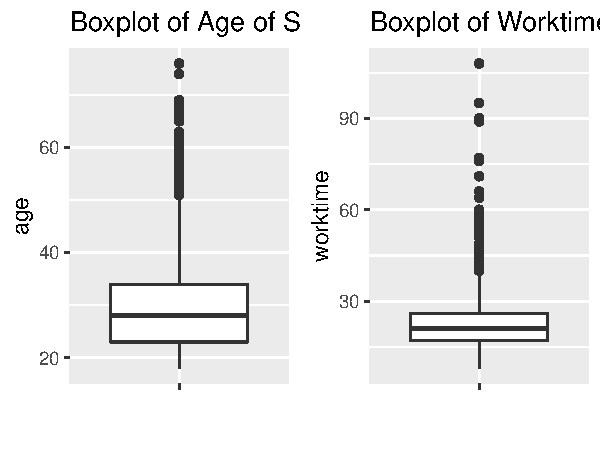
\includegraphics{hw1_sp2022_files/figure-latex/unnamed-chunk-10-1.pdf}

Unlike age and worktime, gender is a categorical variable and thus is
better represented using a histogram instead of a boxplot. We can see
that there are almost 33\% more men which took the survey than women,
potentially meaning there are more male survey workers (although it's
far from conclusive).

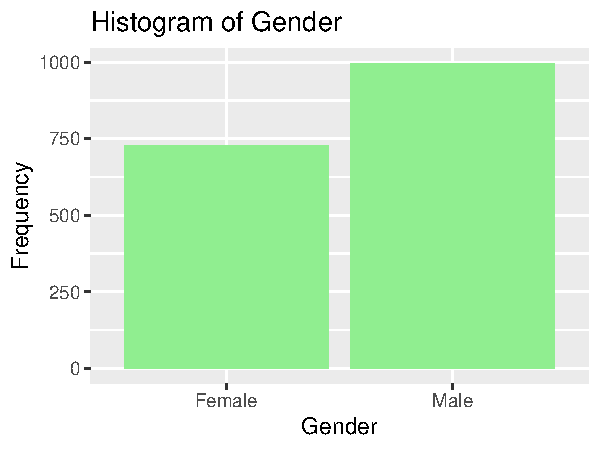
\includegraphics{hw1_sp2022_files/figure-latex/unnamed-chunk-11-1.pdf}

For education and income, both discrete categorical variables, it makes
sense to also create histograms to evaluate the distribution of the
data. We can see that our data most heavily consists of 4-year college
graduates and (likely) many current college students as well as those
who did not finish college or those with an associate's degree. Our data
is more evenly distributed by income group, with the least amount of
respondents in the highest income level (\textgreater{} \$150,000),
which makes sense given they are the population least incentivized by a
job that pays 10 cents per survey.

\begin{verbatim}
## Warning in grid.Call(C_textBounds, as.graphicsAnnot(x$label), x$x, x$y, :
## conversion failure on 'Bachelor’s' in 'mbcsToSbcs': dot substituted for
## <e2>
\end{verbatim}

\begin{verbatim}
## Warning in grid.Call(C_textBounds, as.graphicsAnnot(x$label), x$x, x$y, :
## conversion failure on 'Bachelor’s' in 'mbcsToSbcs': dot substituted for
## <80>
\end{verbatim}

\begin{verbatim}
## Warning in grid.Call(C_textBounds, as.graphicsAnnot(x$label), x$x, x$y, :
## conversion failure on 'Bachelor’s' in 'mbcsToSbcs': dot substituted for
## <99>
\end{verbatim}

\begin{verbatim}
## Warning in grid.Call(C_textBounds, as.graphicsAnnot(x$label), x$x, x$y, :
## conversion failure on 'Associate’s' in 'mbcsToSbcs': dot substituted for
## <e2>
\end{verbatim}

\begin{verbatim}
## Warning in grid.Call(C_textBounds, as.graphicsAnnot(x$label), x$x, x$y, :
## conversion failure on 'Associate’s' in 'mbcsToSbcs': dot substituted for
## <80>
\end{verbatim}

\begin{verbatim}
## Warning in grid.Call(C_textBounds, as.graphicsAnnot(x$label), x$x, x$y, :
## conversion failure on 'Associate’s' in 'mbcsToSbcs': dot substituted for
## <99>
\end{verbatim}

\begin{verbatim}
## Warning in grid.Call(C_textBounds, as.graphicsAnnot(x$label), x$x, x$y, :
## conversion failure on 'Bachelor’s' in 'mbcsToSbcs': dot substituted for
## <e2>
\end{verbatim}

\begin{verbatim}
## Warning in grid.Call(C_textBounds, as.graphicsAnnot(x$label), x$x, x$y, :
## conversion failure on 'Bachelor’s' in 'mbcsToSbcs': dot substituted for
## <80>
\end{verbatim}

\begin{verbatim}
## Warning in grid.Call(C_textBounds, as.graphicsAnnot(x$label), x$x, x$y, :
## conversion failure on 'Bachelor’s' in 'mbcsToSbcs': dot substituted for
## <99>
\end{verbatim}

\begin{verbatim}
## Warning in grid.Call(C_textBounds, as.graphicsAnnot(x$label), x$x, x$y, :
## conversion failure on 'Associate’s' in 'mbcsToSbcs': dot substituted for
## <e2>
\end{verbatim}

\begin{verbatim}
## Warning in grid.Call(C_textBounds, as.graphicsAnnot(x$label), x$x, x$y, :
## conversion failure on 'Associate’s' in 'mbcsToSbcs': dot substituted for
## <80>
\end{verbatim}

\begin{verbatim}
## Warning in grid.Call(C_textBounds, as.graphicsAnnot(x$label), x$x, x$y, :
## conversion failure on 'Associate’s' in 'mbcsToSbcs': dot substituted for
## <99>
\end{verbatim}

\begin{verbatim}
## Warning in grid.Call(C_textBounds, as.graphicsAnnot(x$label), x$x, x$y, :
## conversion failure on 'Bachelor’s' in 'mbcsToSbcs': dot substituted for
## <e2>
\end{verbatim}

\begin{verbatim}
## Warning in grid.Call(C_textBounds, as.graphicsAnnot(x$label), x$x, x$y, :
## conversion failure on 'Bachelor’s' in 'mbcsToSbcs': dot substituted for
## <80>
\end{verbatim}

\begin{verbatim}
## Warning in grid.Call(C_textBounds, as.graphicsAnnot(x$label), x$x, x$y, :
## conversion failure on 'Bachelor’s' in 'mbcsToSbcs': dot substituted for
## <99>
\end{verbatim}

\begin{verbatim}
## Warning in grid.Call(C_textBounds, as.graphicsAnnot(x$label), x$x, x$y, :
## conversion failure on 'Associate’s' in 'mbcsToSbcs': dot substituted for
## <e2>
\end{verbatim}

\begin{verbatim}
## Warning in grid.Call(C_textBounds, as.graphicsAnnot(x$label), x$x, x$y, :
## conversion failure on 'Associate’s' in 'mbcsToSbcs': dot substituted for
## <80>
\end{verbatim}

\begin{verbatim}
## Warning in grid.Call(C_textBounds, as.graphicsAnnot(x$label), x$x, x$y, :
## conversion failure on 'Associate’s' in 'mbcsToSbcs': dot substituted for
## <99>
\end{verbatim}

\begin{verbatim}
## Warning in grid.Call(C_textBounds, as.graphicsAnnot(x$label), x$x, x$y, :
## conversion failure on 'Bachelor’s' in 'mbcsToSbcs': dot substituted for
## <e2>
\end{verbatim}

\begin{verbatim}
## Warning in grid.Call(C_textBounds, as.graphicsAnnot(x$label), x$x, x$y, :
## conversion failure on 'Bachelor’s' in 'mbcsToSbcs': dot substituted for
## <80>
\end{verbatim}

\begin{verbatim}
## Warning in grid.Call(C_textBounds, as.graphicsAnnot(x$label), x$x, x$y, :
## conversion failure on 'Bachelor’s' in 'mbcsToSbcs': dot substituted for
## <99>
\end{verbatim}

\begin{verbatim}
## Warning in grid.Call(C_textBounds, as.graphicsAnnot(x$label), x$x, x$y, :
## conversion failure on 'Associate’s' in 'mbcsToSbcs': dot substituted for
## <e2>
\end{verbatim}

\begin{verbatim}
## Warning in grid.Call(C_textBounds, as.graphicsAnnot(x$label), x$x, x$y, :
## conversion failure on 'Associate’s' in 'mbcsToSbcs': dot substituted for
## <80>
\end{verbatim}

\begin{verbatim}
## Warning in grid.Call(C_textBounds, as.graphicsAnnot(x$label), x$x, x$y, :
## conversion failure on 'Associate’s' in 'mbcsToSbcs': dot substituted for
## <99>
\end{verbatim}

\begin{verbatim}
## Warning in grid.Call(C_textBounds, as.graphicsAnnot(x$label), x$x, x$y, :
## conversion failure on 'Bachelor’s' in 'mbcsToSbcs': dot substituted for
## <e2>
\end{verbatim}

\begin{verbatim}
## Warning in grid.Call(C_textBounds, as.graphicsAnnot(x$label), x$x, x$y, :
## conversion failure on 'Bachelor’s' in 'mbcsToSbcs': dot substituted for
## <80>
\end{verbatim}

\begin{verbatim}
## Warning in grid.Call(C_textBounds, as.graphicsAnnot(x$label), x$x, x$y, :
## conversion failure on 'Bachelor’s' in 'mbcsToSbcs': dot substituted for
## <99>
\end{verbatim}

\begin{verbatim}
## Warning in grid.Call(C_textBounds, as.graphicsAnnot(x$label), x$x, x$y, :
## conversion failure on 'Associate’s' in 'mbcsToSbcs': dot substituted for
## <e2>
\end{verbatim}

\begin{verbatim}
## Warning in grid.Call(C_textBounds, as.graphicsAnnot(x$label), x$x, x$y, :
## conversion failure on 'Associate’s' in 'mbcsToSbcs': dot substituted for
## <80>
\end{verbatim}

\begin{verbatim}
## Warning in grid.Call(C_textBounds, as.graphicsAnnot(x$label), x$x, x$y, :
## conversion failure on 'Associate’s' in 'mbcsToSbcs': dot substituted for
## <99>
\end{verbatim}

\begin{verbatim}
## Warning in grid.Call(C_textBounds, as.graphicsAnnot(x$label), x$x, x$y, :
## conversion failure on 'Bachelor’s' in 'mbcsToSbcs': dot substituted for
## <e2>
\end{verbatim}

\begin{verbatim}
## Warning in grid.Call(C_textBounds, as.graphicsAnnot(x$label), x$x, x$y, :
## conversion failure on 'Bachelor’s' in 'mbcsToSbcs': dot substituted for
## <80>
\end{verbatim}

\begin{verbatim}
## Warning in grid.Call(C_textBounds, as.graphicsAnnot(x$label), x$x, x$y, :
## conversion failure on 'Bachelor’s' in 'mbcsToSbcs': dot substituted for
## <99>
\end{verbatim}

\begin{verbatim}
## Warning in grid.Call(C_textBounds, as.graphicsAnnot(x$label), x$x, x$y, :
## conversion failure on 'Associate’s' in 'mbcsToSbcs': dot substituted for
## <e2>
\end{verbatim}

\begin{verbatim}
## Warning in grid.Call(C_textBounds, as.graphicsAnnot(x$label), x$x, x$y, :
## conversion failure on 'Associate’s' in 'mbcsToSbcs': dot substituted for
## <80>
\end{verbatim}

\begin{verbatim}
## Warning in grid.Call(C_textBounds, as.graphicsAnnot(x$label), x$x, x$y, :
## conversion failure on 'Associate’s' in 'mbcsToSbcs': dot substituted for
## <99>
\end{verbatim}

\begin{verbatim}
## Warning in grid.Call(C_textBounds, as.graphicsAnnot(x$label), x$x, x$y, :
## conversion failure on 'Bachelor’s' in 'mbcsToSbcs': dot substituted for
## <e2>
\end{verbatim}

\begin{verbatim}
## Warning in grid.Call(C_textBounds, as.graphicsAnnot(x$label), x$x, x$y, :
## conversion failure on 'Bachelor’s' in 'mbcsToSbcs': dot substituted for
## <80>
\end{verbatim}

\begin{verbatim}
## Warning in grid.Call(C_textBounds, as.graphicsAnnot(x$label), x$x, x$y, :
## conversion failure on 'Bachelor’s' in 'mbcsToSbcs': dot substituted for
## <99>
\end{verbatim}

\begin{verbatim}
## Warning in grid.Call(C_textBounds, as.graphicsAnnot(x$label), x$x, x$y, :
## conversion failure on 'Associate’s' in 'mbcsToSbcs': dot substituted for
## <e2>
\end{verbatim}

\begin{verbatim}
## Warning in grid.Call(C_textBounds, as.graphicsAnnot(x$label), x$x, x$y, :
## conversion failure on 'Associate’s' in 'mbcsToSbcs': dot substituted for
## <80>
\end{verbatim}

\begin{verbatim}
## Warning in grid.Call(C_textBounds, as.graphicsAnnot(x$label), x$x, x$y, :
## conversion failure on 'Associate’s' in 'mbcsToSbcs': dot substituted for
## <99>
\end{verbatim}

\begin{verbatim}
## Warning in grid.Call(C_textBounds, as.graphicsAnnot(x$label), x$x, x$y, :
## conversion failure on 'Bachelor’s' in 'mbcsToSbcs': dot substituted for
## <e2>
\end{verbatim}

\begin{verbatim}
## Warning in grid.Call(C_textBounds, as.graphicsAnnot(x$label), x$x, x$y, :
## conversion failure on 'Bachelor’s' in 'mbcsToSbcs': dot substituted for
## <80>
\end{verbatim}

\begin{verbatim}
## Warning in grid.Call(C_textBounds, as.graphicsAnnot(x$label), x$x, x$y, :
## conversion failure on 'Bachelor’s' in 'mbcsToSbcs': dot substituted for
## <99>
\end{verbatim}

\begin{verbatim}
## Warning in grid.Call(C_textBounds, as.graphicsAnnot(x$label), x$x, x$y, :
## conversion failure on 'Associate’s' in 'mbcsToSbcs': dot substituted for
## <e2>
\end{verbatim}

\begin{verbatim}
## Warning in grid.Call(C_textBounds, as.graphicsAnnot(x$label), x$x, x$y, :
## conversion failure on 'Associate’s' in 'mbcsToSbcs': dot substituted for
## <80>
\end{verbatim}

\begin{verbatim}
## Warning in grid.Call(C_textBounds, as.graphicsAnnot(x$label), x$x, x$y, :
## conversion failure on 'Associate’s' in 'mbcsToSbcs': dot substituted for
## <99>
\end{verbatim}

\begin{verbatim}
## Warning in grid.Call(C_textBounds, as.graphicsAnnot(x$label), x$x, x$y, :
## conversion failure on 'Bachelor’s' in 'mbcsToSbcs': dot substituted for
## <e2>
\end{verbatim}

\begin{verbatim}
## Warning in grid.Call(C_textBounds, as.graphicsAnnot(x$label), x$x, x$y, :
## conversion failure on 'Bachelor’s' in 'mbcsToSbcs': dot substituted for
## <80>
\end{verbatim}

\begin{verbatim}
## Warning in grid.Call(C_textBounds, as.graphicsAnnot(x$label), x$x, x$y, :
## conversion failure on 'Bachelor’s' in 'mbcsToSbcs': dot substituted for
## <99>
\end{verbatim}

\begin{verbatim}
## Warning in grid.Call(C_textBounds, as.graphicsAnnot(x$label), x$x, x$y, :
## conversion failure on 'Associate’s' in 'mbcsToSbcs': dot substituted for
## <e2>
\end{verbatim}

\begin{verbatim}
## Warning in grid.Call(C_textBounds, as.graphicsAnnot(x$label), x$x, x$y, :
## conversion failure on 'Associate’s' in 'mbcsToSbcs': dot substituted for
## <80>
\end{verbatim}

\begin{verbatim}
## Warning in grid.Call(C_textBounds, as.graphicsAnnot(x$label), x$x, x$y, :
## conversion failure on 'Associate’s' in 'mbcsToSbcs': dot substituted for
## <99>
\end{verbatim}

\begin{verbatim}
## Warning in grid.Call(C_textBounds, as.graphicsAnnot(x$label), x$x, x$y, :
## conversion failure on 'Bachelor’s' in 'mbcsToSbcs': dot substituted for
## <e2>
\end{verbatim}

\begin{verbatim}
## Warning in grid.Call(C_textBounds, as.graphicsAnnot(x$label), x$x, x$y, :
## conversion failure on 'Bachelor’s' in 'mbcsToSbcs': dot substituted for
## <80>
\end{verbatim}

\begin{verbatim}
## Warning in grid.Call(C_textBounds, as.graphicsAnnot(x$label), x$x, x$y, :
## conversion failure on 'Bachelor’s' in 'mbcsToSbcs': dot substituted for
## <99>
\end{verbatim}

\begin{verbatim}
## Warning in grid.Call(C_textBounds, as.graphicsAnnot(x$label), x$x, x$y, :
## conversion failure on 'Associate’s' in 'mbcsToSbcs': dot substituted for
## <e2>
\end{verbatim}

\begin{verbatim}
## Warning in grid.Call(C_textBounds, as.graphicsAnnot(x$label), x$x, x$y, :
## conversion failure on 'Associate’s' in 'mbcsToSbcs': dot substituted for
## <80>
\end{verbatim}

\begin{verbatim}
## Warning in grid.Call(C_textBounds, as.graphicsAnnot(x$label), x$x, x$y, :
## conversion failure on 'Associate’s' in 'mbcsToSbcs': dot substituted for
## <99>
\end{verbatim}

\begin{verbatim}
## Warning in grid.Call(C_textBounds, as.graphicsAnnot(x$label), x$x, x$y, :
## conversion failure on 'Bachelor’s' in 'mbcsToSbcs': dot substituted for
## <e2>
\end{verbatim}

\begin{verbatim}
## Warning in grid.Call(C_textBounds, as.graphicsAnnot(x$label), x$x, x$y, :
## conversion failure on 'Bachelor’s' in 'mbcsToSbcs': dot substituted for
## <80>
\end{verbatim}

\begin{verbatim}
## Warning in grid.Call(C_textBounds, as.graphicsAnnot(x$label), x$x, x$y, :
## conversion failure on 'Bachelor’s' in 'mbcsToSbcs': dot substituted for
## <99>
\end{verbatim}

\begin{verbatim}
## Warning in grid.Call(C_textBounds, as.graphicsAnnot(x$label), x$x, x$y, :
## conversion failure on 'Associate’s' in 'mbcsToSbcs': dot substituted for
## <e2>
\end{verbatim}

\begin{verbatim}
## Warning in grid.Call(C_textBounds, as.graphicsAnnot(x$label), x$x, x$y, :
## conversion failure on 'Associate’s' in 'mbcsToSbcs': dot substituted for
## <80>
\end{verbatim}

\begin{verbatim}
## Warning in grid.Call(C_textBounds, as.graphicsAnnot(x$label), x$x, x$y, :
## conversion failure on 'Associate’s' in 'mbcsToSbcs': dot substituted for
## <99>
\end{verbatim}

\begin{verbatim}
## Warning in grid.Call(C_textBounds, as.graphicsAnnot(x$label), x$x, x$y, :
## conversion failure on 'Bachelor’s' in 'mbcsToSbcs': dot substituted for
## <e2>
\end{verbatim}

\begin{verbatim}
## Warning in grid.Call(C_textBounds, as.graphicsAnnot(x$label), x$x, x$y, :
## conversion failure on 'Bachelor’s' in 'mbcsToSbcs': dot substituted for
## <80>
\end{verbatim}

\begin{verbatim}
## Warning in grid.Call(C_textBounds, as.graphicsAnnot(x$label), x$x, x$y, :
## conversion failure on 'Bachelor’s' in 'mbcsToSbcs': dot substituted for
## <99>
\end{verbatim}

\begin{verbatim}
## Warning in grid.Call(C_textBounds, as.graphicsAnnot(x$label), x$x, x$y, :
## conversion failure on 'Associate’s' in 'mbcsToSbcs': dot substituted for
## <e2>
\end{verbatim}

\begin{verbatim}
## Warning in grid.Call(C_textBounds, as.graphicsAnnot(x$label), x$x, x$y, :
## conversion failure on 'Associate’s' in 'mbcsToSbcs': dot substituted for
## <80>
\end{verbatim}

\begin{verbatim}
## Warning in grid.Call(C_textBounds, as.graphicsAnnot(x$label), x$x, x$y, :
## conversion failure on 'Associate’s' in 'mbcsToSbcs': dot substituted for
## <99>
\end{verbatim}

\begin{verbatim}
## Warning in grid.Call(C_textBounds, as.graphicsAnnot(x$label), x$x, x$y, :
## conversion failure on 'Bachelor’s' in 'mbcsToSbcs': dot substituted for
## <e2>
\end{verbatim}

\begin{verbatim}
## Warning in grid.Call(C_textBounds, as.graphicsAnnot(x$label), x$x, x$y, :
## conversion failure on 'Bachelor’s' in 'mbcsToSbcs': dot substituted for
## <80>
\end{verbatim}

\begin{verbatim}
## Warning in grid.Call(C_textBounds, as.graphicsAnnot(x$label), x$x, x$y, :
## conversion failure on 'Bachelor’s' in 'mbcsToSbcs': dot substituted for
## <99>
\end{verbatim}

\begin{verbatim}
## Warning in grid.Call(C_textBounds, as.graphicsAnnot(x$label), x$x, x$y, :
## conversion failure on 'Associate’s' in 'mbcsToSbcs': dot substituted for
## <e2>
\end{verbatim}

\begin{verbatim}
## Warning in grid.Call(C_textBounds, as.graphicsAnnot(x$label), x$x, x$y, :
## conversion failure on 'Associate’s' in 'mbcsToSbcs': dot substituted for
## <80>
\end{verbatim}

\begin{verbatim}
## Warning in grid.Call(C_textBounds, as.graphicsAnnot(x$label), x$x, x$y, :
## conversion failure on 'Associate’s' in 'mbcsToSbcs': dot substituted for
## <99>
\end{verbatim}

\begin{verbatim}
## Warning in grid.Call.graphics(C_text, as.graphicsAnnot(x$label), x$x,
## x$y, : conversion failure on 'Bachelor’s' in 'mbcsToSbcs': dot substituted
## for <e2>
\end{verbatim}

\begin{verbatim}
## Warning in grid.Call.graphics(C_text, as.graphicsAnnot(x$label), x$x,
## x$y, : conversion failure on 'Bachelor’s' in 'mbcsToSbcs': dot substituted
## for <80>
\end{verbatim}

\begin{verbatim}
## Warning in grid.Call.graphics(C_text, as.graphicsAnnot(x$label), x$x,
## x$y, : conversion failure on 'Bachelor’s' in 'mbcsToSbcs': dot substituted
## for <99>
\end{verbatim}

\begin{verbatim}
## Warning in grid.Call.graphics(C_text, as.graphicsAnnot(x$label), x$x,
## x$y, : conversion failure on 'Associate’s' in 'mbcsToSbcs': dot substituted
## for <e2>
\end{verbatim}

\begin{verbatim}
## Warning in grid.Call.graphics(C_text, as.graphicsAnnot(x$label), x$x,
## x$y, : conversion failure on 'Associate’s' in 'mbcsToSbcs': dot substituted
## for <80>
\end{verbatim}

\begin{verbatim}
## Warning in grid.Call.graphics(C_text, as.graphicsAnnot(x$label), x$x,
## x$y, : conversion failure on 'Associate’s' in 'mbcsToSbcs': dot substituted
## for <99>
\end{verbatim}

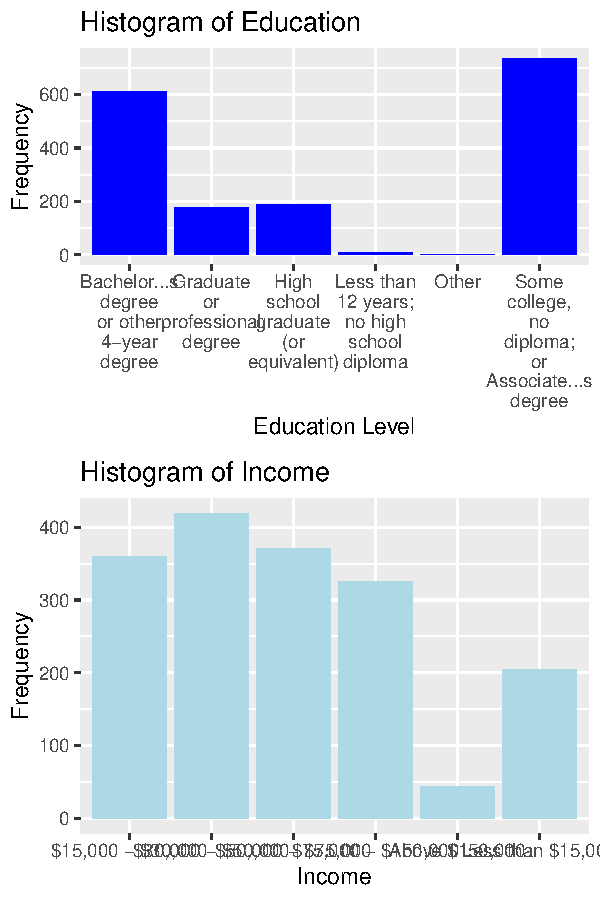
\includegraphics{hw1_sp2022_files/figure-latex/unnamed-chunk-12-1.pdf}

Lastly, we can represent the listening habits of histograms as well
given that they're also discrete categorical variables. From the graphs,
it's evident that although there are plenty of Sirius listeners in the
survey workers, there are few people which have listen Sirius Business
Radio by Wharton.

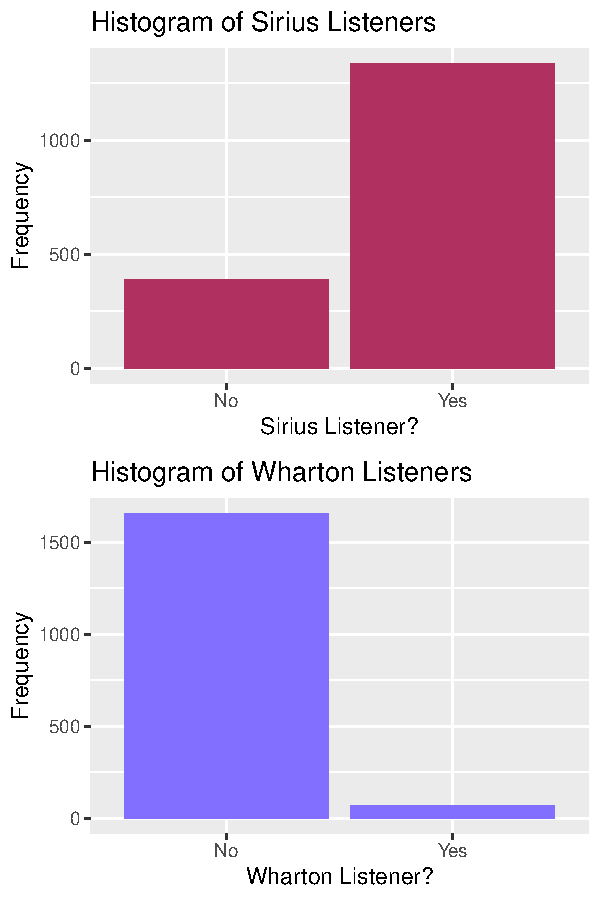
\includegraphics{hw1_sp2022_files/figure-latex/unnamed-chunk-13-1.pdf}

\hypertarget{sample-properties}{%
\subsection{Sample properties}\label{sample-properties}}

The population from which the sample is drawn determines where the
results of our analysis can be applied or generalized. We include some
basic demographic information for the purpose of identifying sample
bias, if any exists. Combine our data and the general population
distribution in age, gender and income to try to characterize our sample
on hand.

\begin{enumerate}
\def\labelenumi{\roman{enumi}.}
\tightlist
\item
  Does this sample appear to be a random sample from the general
  population of the USA?
\end{enumerate}

In terms of gender, this sample does not appear to be a random sample
from the general population of the US given the disproportionate number
of males compared to females given that in the US there are actually
more women than men (161.7 million vs 156.7 million in 2014). The income
distributions are more realistic of the US population given that the
median income levels in our age group are around \$30,000-50,000
(\url{https://dqydj.com/average-median-top-income-by-age-percentiles/})
which is not only the mode of our distribution, but the ranges around it
are also highly populated. When comparing our education data to the
distribution in the US
(\url{https://www.statista.com/statistics/785618/educational-attainment-by-age-group-us/}),
we can see that our sample is more educated given the larger percentage
of those with at least a bachelor's degree and disproportionally small
number of people with less than a high school diploma (\textless1\%
instead of around 10\%) and those with only a high school diploma (11\%
instead of around 26-33\%).

This sample does not seem to be a representative random sample of the
general population, as the sample is skewed younger and within that age
group, it is more male heavy and more educated.

\begin{enumerate}
\def\labelenumi{\roman{enumi}.}
\setcounter{enumi}{1}
\tightlist
\item
  Does this sample appear to be a random sample from the MTURK
  population?
\end{enumerate}

When considering the general MTURK population, we again see that our
sample has a disproportionate number of men instead of women given that
across each age group, there are actually more female participants on
MTURK. However, it is important to note that the older MTURK workers are
most heavily concentrated with females and our data consists of mostly
younger people. This sample does seem to be representative age-wise of
the relatively young MTURK population, as most data entries are for
people under 40. As pointed out on the website from which we pull this
MTURK data
(\url{https://www.cloudresearch.com/resources/blog/who-uses-amazon-mturk-2020-demographics/}),
the distribution of income is similar to that of the US population,
which we have already noted is similarly represented in our sample. For
education, it does seem like our data is similar to the distribution of
education levels among US MTURK workers
(\url{https://crowdsourcing-class.org/readings/downloads/platform/demographics-of-mturk.pdf}).
It does seem like this sample is a representative random sample from the
MTURK population outside of the gender distribution.

Note: You can not provide evidence by simply looking at our data here.
For example, you need to find distribution of education in our age group
in US to see if the two groups match in distribution. You may need to
gather some background information about the MTURK population to have a
slight sense if this particular sample seem to a random sample from
there\ldots{} Please do not spend too much time gathering evidence.

\hypertarget{final-estimate}{%
\subsection{Final estimate}\label{final-estimate}}

Give a final estimate of the Wharton audience size in January 2014.
Assume that the sample is a random sample of the MTURK population, and
that the proportion of Wharton listeners vs.~Sirius listeners in the
general population is the same as that in the MTURK population. Write a
brief executive summary to summarize your findings and how you came to
that conclusion.

To be specific, you should include:

\begin{enumerate}
\def\labelenumi{\arabic{enumi}.}
\tightlist
\item
  Goal of the study
\item
  Method used: data gathering, estimation methods
\item
  Findings
\item
  Limitations of the study.
\end{enumerate}

Before writing the executive summary, we need to first estimate the
Wharton audience using the proportion p of Wharton Sirius listeners from
our dataset.

\textbf{Executive summary:} We conducted a study to measure the success
of the Wharton Talk Show on Sirius Radio, that is, estimate the number
of listeners. We got our data from a survey we launched on Amazon
Mechanical Turk (MTURK) in May 2014 which included basic demographic
questions and asked repondents whether they were a Sirius Radio listener
and if they have listened to Sirius Business Radio by Wharton. We ended
up with a random sample of 1,725 responses from the MTURK population, a
population which we assumed shares the same proportion of Wharton
listeners vs.~Sirius listeners in the general population. Therefore, to
estimate the audience size for the Wharton Talk Show, we calculated the
proportion (p) of Sirius listeners which have listened to the Wharton
show and got about 5\%. We then multiplied that p value by 51.6 million,
overall number of Sirius listeners to get an estimated approximate
audience size of 2,587,725 people. Our study is not without limitations
however, given that it is very dependent on our assumption about the
consistency of our sample compared to the population of Sirius
listeners. There is no evidence to support this and our sample is shown
to be somewhat differently distributed than the US population of the
same age range. We are also making inferences on a population of 51.6
million listeners based on less than 2000 people, which is a large
claim.

\hypertarget{new-task}{%
\subsection{New task}\label{new-task}}

Now suppose you are asked to design a study to estimate the audience
size of Wharton Business Radio Show as of today: You are given a budget
of \$1000. You need to present your findings in two months.

Write a proposal for this study which includes:

\begin{enumerate}
\def\labelenumi{\arabic{enumi}.}
\tightlist
\item
  Method proposed to estimate the audience size.
\item
  What data should be collected and where it should be sourced from.
  Please fill in the google form to list your platform where surveys
  will be launched and collected
  \href{https://forms.gle/8SmjFQ1tpqr6c4sa8}{HERE}
\end{enumerate}

A good proposal will give an accurate estimation with the least amount
of money used.

\textbf{Answer:} For the new survey, we immediately wanted to account
for the fact that Wharton Business Radio is not exclusive to SiriusXM
anymore, given that clips are available for listening or download online
and it's also available on platforms like Apple Music. For this reason,
instead of estimating the proportion p of Sirius listeners that listen
to Wharton Business Radio, we want to expand to estimate the proportion
of the general US population which have listened to the show. To collect
this random sampling of US citizens, we would like to use the platform
which brings together a wide variety of characters: Twitter. We would
like to create a free survey on Qualtrics that we would link in the
Twitter promoted tweet which we would limit geographically to the US and
age-wise to those above the age of 16. The survey would have the same
questions as the original study from 2014, besides the question on
whether the person is a Sirius listener and instead include a drop-down
question on where they listened to the show. While this won't help with
our prediction, it would support our hypothesis that Wharton Business
Radio listeners are not limited to SiriusXM subscribers and improve on
the original study.

Twitter gave an estimate that there would be a cost of \$0.50 per
interaction, and aiming for 2,000 responses, the total cost of data
collection would then be \$1000. We would also only leave the ad and
survey open for 1 month to collect the data and provide an additional
month for us to analyze and put together our findings.

\hypertarget{case-study-2-women-in-science}{%
\section{Case study 2: Women in
Science}\label{case-study-2-women-in-science}}

Are women underrepresented in science in general? How does gender relate
to the type of educational degree pursued? Does the number of higher
degrees increase over the years? In an attempt to answer these
questions, we assembled a data set (\texttt{WomenData\_06\_16.xlsx})
from
\href{https://ncses.nsf.gov/pubs/nsf19304/digest/field-of-degree-women}{NSF}
about various degrees granted in the U.S. from 2006 to 2016. It contains
the following variables: Field (Non-science-engineering
(\texttt{Non-S\&E}) and sciences (\texttt{Computer\ sciences},
\texttt{Mathematics\ and\ statistics}, etc.)), Degree (\texttt{BS},
\texttt{MS}, \texttt{PhD}), Sex (\texttt{M}, \texttt{F}), Number of
degrees granted, and Year.

Our goal is to answer the above questions only through EDA (Exploratory
Data Analyses) without formal testing. We have provided sample R-codes
in the appendix to help you if needed.

\hypertarget{data-preparation-1}{%
\subsection{Data preparation}\label{data-preparation-1}}

\begin{enumerate}
\def\labelenumi{\arabic{enumi}.}
\tightlist
\item
  Understand and clean the data
\end{enumerate}

Notice the data came in as an Excel file. We need to use the package
\texttt{readxl} and the function \texttt{read\_excel()} to read the data
\texttt{WomenData\_06\_16.xlsx} into R.

\begin{enumerate}
\def\labelenumi{\roman{enumi}.}
\item
  Read the data into R.
\item
  Clean the names of each variables. (Change variable names to
  \texttt{Field},\texttt{Degree}, \texttt{Sex}, \texttt{Year} and
  \texttt{Number} )
\item
  Set the variable natures properly.
\item
  Any missing values?
\end{enumerate}

\textbf{Answer:} There are no missing values.

\begin{enumerate}
\def\labelenumi{\arabic{enumi}.}
\setcounter{enumi}{1}
\tightlist
\item
  Write a summary describing the data set provided here.
\end{enumerate}

\begin{enumerate}
\def\labelenumi{\roman{enumi}.}
\tightlist
\item
  How many fields are there in this data?
\item
  What are the degree types?
\item
  How many year's statistics are being reported here?
\end{enumerate}

\textbf{Answer:} In this data, there are 660 different entries and 5
different variables: Field, Degree, Sex, Year, and Number. Within the
Field variable, there are 10 distinct fields. The different degree types
are BS, MS, and PhD. There are 11 years of statistics reported with the
data spanning from 2006-2016. The minimum number of degrees awarded for
a single degree type and for a particular sex in a year is 218, while
the max is 781474.

\hypertarget{bs-degrees-in-2015}{%
\subsection{BS degrees in 2015}\label{bs-degrees-in-2015}}

Is there evidence that more males are in science-related fields vs
\texttt{Non-S\&E}? Provide summary statistics and a plot which shows the
number of people by gender and by field. Write a brief summary to
describe your findings.

\includegraphics{hw1_sp2022_files/figure-latex/unnamed-chunk-23-1.pdf}
\includegraphics{hw1_sp2022_files/figure-latex/unnamed-chunk-23-2.pdf}

\textbf{Answer:} Only looking at the histogram side for male (not
comparing to the female side), there is no evidence that there are more
males in science-related fields than males in non-S\&E. In fact, there
are around 1.5 times as many males in non-S\&E than there are in
science-related fields. There is a similar trend when looking at the
female side. However, there is a greater difference of females in
Non-S\&E than science-related. This greater difference is largely due to
there being more female in Non-S\&E fields than there are male since the
number of female and male in science-related fields is roughly equal.
Comparatively to the ratio of female in science-related fields vs
Non-S\&E, there are more male in science-related fields vs Non-S\&E.

\hypertarget{eda-bringing-type-of-degree-field-and-gender-in-2015}{%
\subsection{EDA bringing type of degree, field and gender in
2015}\label{eda-bringing-type-of-degree-field-and-gender-in-2015}}

Describe the number of people by type of degree, field, and gender. Do
you see any evidence of gender effects over different types of degrees?
Again, provide graphs to summarize your findings.

\includegraphics{hw1_sp2022_files/figure-latex/unnamed-chunk-24-1.pdf}
\includegraphics{hw1_sp2022_files/figure-latex/unnamed-chunk-24-2.pdf}
\includegraphics{hw1_sp2022_files/figure-latex/unnamed-chunk-24-3.pdf}

\textbf{Answer:} Within the Non-S\&E fields, there is consistently more
degrees awarded to females than males (about double as much) across all
types of degrees so there is evidence of a general gender effect over
all Non-S\&E field degrees that more are awarded to females but no
evidence that the gender effect changes based on degree type. However,
with science-related fields, the gap between degrees awarded to females
and males widens the higher the degree is. For the BS degree, there is
roughly an equal amount of degrees awarded to each sex, with a little
more to female than male. However, for the MS degree, there is about
double as many degrees awarded to male than female. This difference is
replicated in the PhD degree. Therefore, because of the difference of
degrees awarded to each sex in MS and PhD degrees but lack of difference
in BS degree, there is evidence of gender effects over the MS and PhD
degrees that more degrees are awarded to males (about twice as much).

\hypertarget{eda-bring-all-variables}{%
\subsection{EDA bring all variables}\label{eda-bring-all-variables}}

In this last portion of the EDA, we ask you to provide evidence
numerically and graphically: Do the number of degrees change by gender,
field, and time?

\begin{verbatim}
## `summarise()` has grouped output by 'ScienceField'. You can override using the `.groups` argument.
\end{verbatim}

\begin{verbatim}
## `summarise()` has grouped output by 'ScienceField', 'Sex'. You can override using the `.groups` argument.
\end{verbatim}

\begin{verbatim}
## `summarise()` has grouped output by 'ScienceField', 'Sex', 'Year'. You can override using the `.groups` argument.
\end{verbatim}

\includegraphics{hw1_sp2022_files/figure-latex/unnamed-chunk-25-1.pdf}

\begin{verbatim}
## `summarise()` has grouped output by 'ScienceField', 'Sex', 'Year'. You can override using the `.groups` argument.
\end{verbatim}

\includegraphics{hw1_sp2022_files/figure-latex/unnamed-chunk-25-2.pdf}

\begin{verbatim}
## `summarise()` has grouped output by 'ScienceField', 'Sex'. You can override using the `.groups` argument.
\end{verbatim}

\includegraphics{hw1_sp2022_files/figure-latex/unnamed-chunk-25-3.pdf}

\begin{verbatim}
## `summarise()` has grouped output by 'ScienceField', 'Sex', 'Year'. You can override using the `.groups` argument.
\end{verbatim}

\includegraphics{hw1_sp2022_files/figure-latex/unnamed-chunk-25-4.pdf}

\textbf{Answer:} For Non-S\&E fields, there have consistently been about
1.5 as many female as male receiving degrees throughout the years and
degree types (with a little less of a difference in PhD than BS). For
science-related fields, there have consistently throughout the years
been an equal amount of BS degrees awarded, a slightly higher amount of
MS degrees awarded for males, and a slightly higher amount than seen in
the MS degrees in PhD degrees. When looking at the trend for female
proportion across the years for each field type, females make up more
than 60\% of the proportion in Non-S\&E fields throughout all the years,
but make up less than 50\% of the proportion in science-related fields.
In the more recent years (2014-2016), the proportion of females in
science-related fields have decreased but have increased for Non-S\&E.
These trends are more exaggerated when separating the different degree
types. Females are least represented throughout the years in
science-related fields when looking at PhD degrees (41\%), while they
are about equally represented in BS degrees (50\%) and in between BS and
PhD representation for MS degrees (45\%). Female proportion in Non-S\&E
are similar throughout the years for BS and PhD degrees at about 61\%
(although less consistent for PhD), while proportion in MS degrees is a
bit higher at 64\%.

\hypertarget{women-in-data-science}{%
\subsection{Women in Data Science}\label{women-in-data-science}}

Finally, is there evidence showing that women are underrepresented in
data science? Data science is an interdisciplinary field of computer
science, math, and statistics. You may include year and/or degree.

\includegraphics{hw1_sp2022_files/figure-latex/unnamed-chunk-26-1.pdf}
\includegraphics{hw1_sp2022_files/figure-latex/unnamed-chunk-26-2.pdf}

\textbf{Answer:} There is evidence of women being underrepresented in
data science as there is a large difference in the number of computer
science or math and statistics degrees awarded to males compared to
females. This difference is about 5 times as much for BS degrees, twice
as much for MS degrees, and 4 times as much for PhD degrees. Overall,
degrees in computer science or math and statistics are awarded about 4-5
times more to males than females.

\hypertarget{final-brief-report}{%
\subsection{Final brief report}\label{final-brief-report}}

Summarize your findings focusing on answering the questions regarding if
we see consistent patterns that more males pursue science-related
fields. Any concerns with the data set? How could we improve on the
study?

\textbf{Answer:} The proportion of females vs males in science-related
fields have stayed pretty consistent over time, even when separating my
degree type. However, when separating my degree type, the proportion of
females vs males in science-related fields change. The higher the degree
type, the less females there is proportionately receiving degrees. There
is about an equal amount of BS degrees awarded to females as males
(50\%), then there is less MS degrees proportionately awarded (45\%),
and even less PhD degrees proportionately awarded (41\%). As the degree
type increases, there is about a 5\% decrease in representation of
females proportionately to males. Therefore, there is evidence to
suggest that more males pursue science related fields with higher degree
types. One concern with the data set is that the report states ``Surveys
conducted by the National Center for Science and Engineering Statistics
(NCSES) within the National Science Foundation provided a large portion
of the data used in this report'', we wonder if the surveys were
represented of the whole population. We can improve on the study by
looking into other ways to be involved in the sciences besides degrees
like technical school certificates.

\hypertarget{appendix}{%
\subsection{Appendix}\label{appendix}}

To help out, we have included some R-codes here as references. You
should make your own chunks filled with texts going through each items
listed above. Make sure to hide the unnecessary outputs/code etc.

\begin{enumerate}
\def\labelenumi{\arabic{enumi}.}
\item
  Clean data
\item
  A number of sample analyses
\end{enumerate}

\hypertarget{case-study-3-major-league-baseball}{%
\section{Case study 3: Major League
Baseball}\label{case-study-3-major-league-baseball}}

We would like to explore how payroll affects performance among Major
League Baseball teams. The data is prepared in two formats record
payroll, winning numbers/percentage by team from 1998 to 2014.

Here are the datasets:

-\texttt{MLPayData\_Total.csv}: wide format -\texttt{baseball.csv}: long
format

Feel free to use either dataset to address the problems.

\begin{verbatim}
## Parsed with column specification:
## cols(
##   team = col_character(),
##   year = col_double(),
##   payroll = col_double(),
##   win_num = col_double(),
##   win_pct = col_double()
## )
\end{verbatim}

\begin{verbatim}
## Parsed with column specification:
## cols(
##   .default = col_double(),
##   Team.name.2014 = col_character()
## )
\end{verbatim}

\begin{verbatim}
## See spec(...) for full column specifications.
\end{verbatim}

\hypertarget{eda-relationship-between-payroll-changes-and-performance}{%
\subsection{EDA: Relationship between payroll changes and
performance}\label{eda-relationship-between-payroll-changes-and-performance}}

Payroll may relate to performance among ML Baseball teams. One possible
argument is that what affects this year's performance is not this year's
payroll, but the amount that payroll increased from last year. Let us
look into this through EDA.

Create increment in payroll

\begin{enumerate}
\def\labelenumi{\roman{enumi}.}
\item
  To describe the increment of payroll in each year there are several
  possible approaches. Take 2013 as an example:

  \begin{itemize}
  \tightlist
  \item
    option 1: diff: payroll\_2013 - payroll\_2012
  \item
    option 2: log diff: log(payroll\_2013) - log(payroll\_2012)
  \end{itemize}
\end{enumerate}

Explain why the log difference is more appropriate in this setup.

\textbf{Answer:} We want to use the log difference as it allows us to
approximate the percent change in the payroll rather than just the
difference in pay. By converting the differences to the log scale we can
compare the different teams on a more standardized scale. This allows us
to level our the teams that get more funding to those with less funding.

\begin{enumerate}
\def\labelenumi{\roman{enumi}.}
\setcounter{enumi}{1}
\item
  Create a new variable
  \texttt{diff\_log=log(payroll\_2013)\ -\ log(payroll\_2012)}. Hint:
  use \texttt{dplyr::lag()} function.
\item
  Create a long data table including: team, year, diff\_log, win\_pct
\end{enumerate}

\hypertarget{exploratory-questions}{%
\subsection{Exploratory questions}\label{exploratory-questions}}

\begin{enumerate}
\def\labelenumi{\roman{enumi}.}
\tightlist
\item
  Which five teams had highest increase in their payroll between years
  2010 and 2014, inclusive?
\end{enumerate}

\textbf{Answer:} The teams with the highest increase in payroll between
2010 and 2014 inclusive are 1. Houston Astros 0.812\\
2. Oakland Athletics 0.506\\
3. Arizona Diamondbacks 0.427\\
4. San Diego Padres 0.418\\
5. Texas Rangers 0.393

\begin{enumerate}
\def\labelenumi{\roman{enumi}.}
\setcounter{enumi}{1}
\tightlist
\item
  Between 2010 and 2014, inclusive, which team(s) ``improved'' the most?
  That is, had the biggest percentage gain in wins?
\end{enumerate}

\textbf{Answer:} The team with the biggest percent change, or that
improved the most from 2010 to 2014 was the Pittsburgh Pirates. Their
percent change was 0.19136.

\hypertarget{do-log-increases-in-payroll-imply-better-performance}{%
\subsection{Do log increases in payroll imply better
performance?}\label{do-log-increases-in-payroll-imply-better-performance}}

Is there evidence to support the hypothesis that higher increases in
payroll on the log scale lead to increased performance? Pick up a few
statistics, accompanied with some data visualization, to support your
answer.

\begin{verbatim}
## Warning: package 'ggrepel' was built under R version 3.5.2
\end{verbatim}

\includegraphics{hw1_sp2022_files/figure-latex/unnamed-chunk-36-1.pdf}
\textbf{Answer:} Based on this graph of the average change in payroll,
(average of diff\_log for each team)and the win percent average over the
years 1998-2014, there does not appear to be any correlation between the
variables. In fact the correlation is nearly zero meaning that those two
variables have little to no effect on one another.

\includegraphics{hw1_sp2022_files/figure-latex/unnamed-chunk-37-1.pdf}

\textbf{Answer:} The correlation between the log difference of the
payroll between years and the win percentage for games that year is very
low. 0.345 indicates there is very low correlation between those
variables.

We can also use the graphs from the prior question to see that the top 5
teams with the greater percent increase in payroll between 2010 and 2014
do not line up with the top 5 teams that had the biggest percent change
in wins from those years

\begin{verbatim}
## Warning: Removed 30 rows containing non-finite values (stat_smooth).
\end{verbatim}

\begin{verbatim}
## Warning: Removed 30 rows containing missing values (geom_point).
\end{verbatim}

\includegraphics{hw1_sp2022_files/figure-latex/unnamed-chunk-38-1.pdf}
\textbf{Answer:} From the plots above, we are able to look at the
changes in payroll on the log scale and the win percentage for group by
each year. We can see that there is no clear positive correlation for
all of the years. Some have a least squares line that is flat, some have
positive, and have negative. This further proves my belief that there is
no relation between change is payroll on the log scale and winning
percentage.

So overall, we can conclude that there is not evidence to support the
hypothesis that higher increases in payroll on the log scale lead to
increased performance. In fact our data showed that there is no
correlation between the payroll increases on the log scale and the
percentage of wins per year for teams

\hypertarget{comparison}{%
\subsection{Comparison}\label{comparison}}

Which set of factors are better explaining performance? Yearly payroll
or yearly increase in payroll? What criterion is being used?

\textbf{Answer:} Yearly Payroll

We can see that Yearly payroll has a higher correlation with win
percentage than the yearly increase in payroll. We can also look at
these plots below to see if there is a visual correlation as well.

\includegraphics{hw1_sp2022_files/figure-latex/unnamed-chunk-40-1.pdf}
\includegraphics{hw1_sp2022_files/figure-latex/unnamed-chunk-40-2.pdf}

Although neither plot indicates a strong correlation between the two
variable, you can see there is a weak positive correlation between
Yearly Payroll and win percentage compared to the other scatter plot of
change in payroll and win percentage that does not indicate any
correlation.

\end{document}
